\documentclass[aspectratio=169,11pt]{beamer}
\usepackage[utf8]{inputenc}
\usepackage[T1]{fontenc}
\usepackage{lmodern}
\usepackage{booktabs}
\usepackage{graphicx}
\graphicspath{{../figures/}}

\usetheme{default}
\setbeamertemplate{navigation symbols}{}
\setbeamertemplate{footline}{\hfill\scriptsize\color{gray}\insertframenumber\,/\,\inserttotalframenumber\hspace{1.2em}\vspace{0.6em}}
\definecolor{accent}{HTML}{4A3AA7}
\definecolor{warn}{HTML}{E34948}
\setbeamercolor{frametitle}{fg=accent}
\setbeamercolor{title}{fg=accent}
\setbeamercolor{structure}{fg=accent}
\setbeamerfont{frametitle}{series=\bfseries,size=\Large}
\setbeamertemplate{itemize item}{\color{accent}\textbullet}
\setbeamertemplate{itemize subitem}{\color{gray}--}

\newcommand{\MD}{M_{\mathrm D}}
\newcommand{\MN}{M_{\mathrm N}}
\newcommand{\WN}{W_{\mathrm N}}
\newcommand{\key}[1]{\textcolor{accent}{\textbf{#1}}}
\newcommand{\bad}[1]{\textcolor{warn}{\textbf{#1}}}

\title{WCS417 drought rescue across 247 \emph{Arabidopsis} accessions}
\subtitle{Reanalysis of the natural-variation screen, including the replicate runs}
\author{Abdul Aziz Eida \and Kundai Farai Sachikonye}
\date{October 2026 \\[0.5em] \footnotesize Unpublished data of the collaborating laboratory --- not for distribution}

\begin{document}

% =====================================================================
\begin{frame}
  \titlepage
\end{frame}

% =====================================================================
\begin{frame}{The question before the GWAS}
  \begin{columns}[T]
    \column{0.52\textwidth}
    \begin{itemize}
      \item The screen is a factorial for every accession:
        \begin{itemize}
          \item mock / WCS417 $\times$ drought / non-stress $\times$ shoot / root.
        \end{itemize}
      \item A GWAS needs \key{one number} per accession.
      \item Six readings were mapped separately:
        \begin{itemize}
          \item biomass, gain, \% increase, \% rescue, \% loss, rescuer label.
        \end{itemize}
      \item Each reading gave different candidate genes, and no accession lost rescue.
    \end{itemize}
    \column{0.44\textwidth}
    \vspace{0.6em}
    \begin{block}{Two questions}
      \begin{enumerate}
        \item Which of these numbers \emph{is} the rescue of an accession?
        \item Does it replicate from one run to the next?
      \end{enumerate}
    \end{block}
    \vspace{0.5em}
    \small Part I answers question 1 from the first workbook. Part II answers question 2
    from the full per-plant workbook.
  \end{columns}
\end{frame}

% =====================================================================
\begin{frame}{The data}
  \begin{columns}[T]
    \column{0.5\textwidth}
    \textbf{First workbook} (GWAS input)
    \begin{itemize}
      \item Per-plant weights for WCS417 + drought only (1,841 plants).
      \item The other cells appear only as averages inside the derived traits.
      \item easyGWAS output: 28 candidate genes, 40 rows.
    \end{itemize}
    \column{0.5\textwidth}
    \textbf{Second workbook} (\texttt{NS+DS.xlsx})
    \begin{itemize}
      \item 8,820 plants: all four cells, 247 accessions.
      \item Drought run 1: all accessions.
      \item Drought runs 2 and 3: 50 accessions,
        \begin{itemize}
          \item 43 of them labelled \emph{non-rescuers}.
        \end{itemize}
      \item Col-0 grown in 7-plant blocks in every cell and run.
    \end{itemize}
  \end{columns}
  \vspace{1em}
  \small Notation: $W$ = WCS417 drought, $\MD$ = mock drought, $\MN$ = mock non-stress,
  $\WN$ = WCS417 non-stress (all cell means).
\end{frame}

% =====================================================================
\section{Part I --- which number is rescue?}
\begin{frame}
  \centering\Large\color{accent}\textbf{Part I}\\[0.4em]
  \normalsize\color{black} Which number is the rescue of an accession?
\end{frame}

% =====================================================================
\begin{frame}{Every derived trait is an exact formula in three cell means}
  \begin{columns}[c]
    \column{0.58\textwidth}
    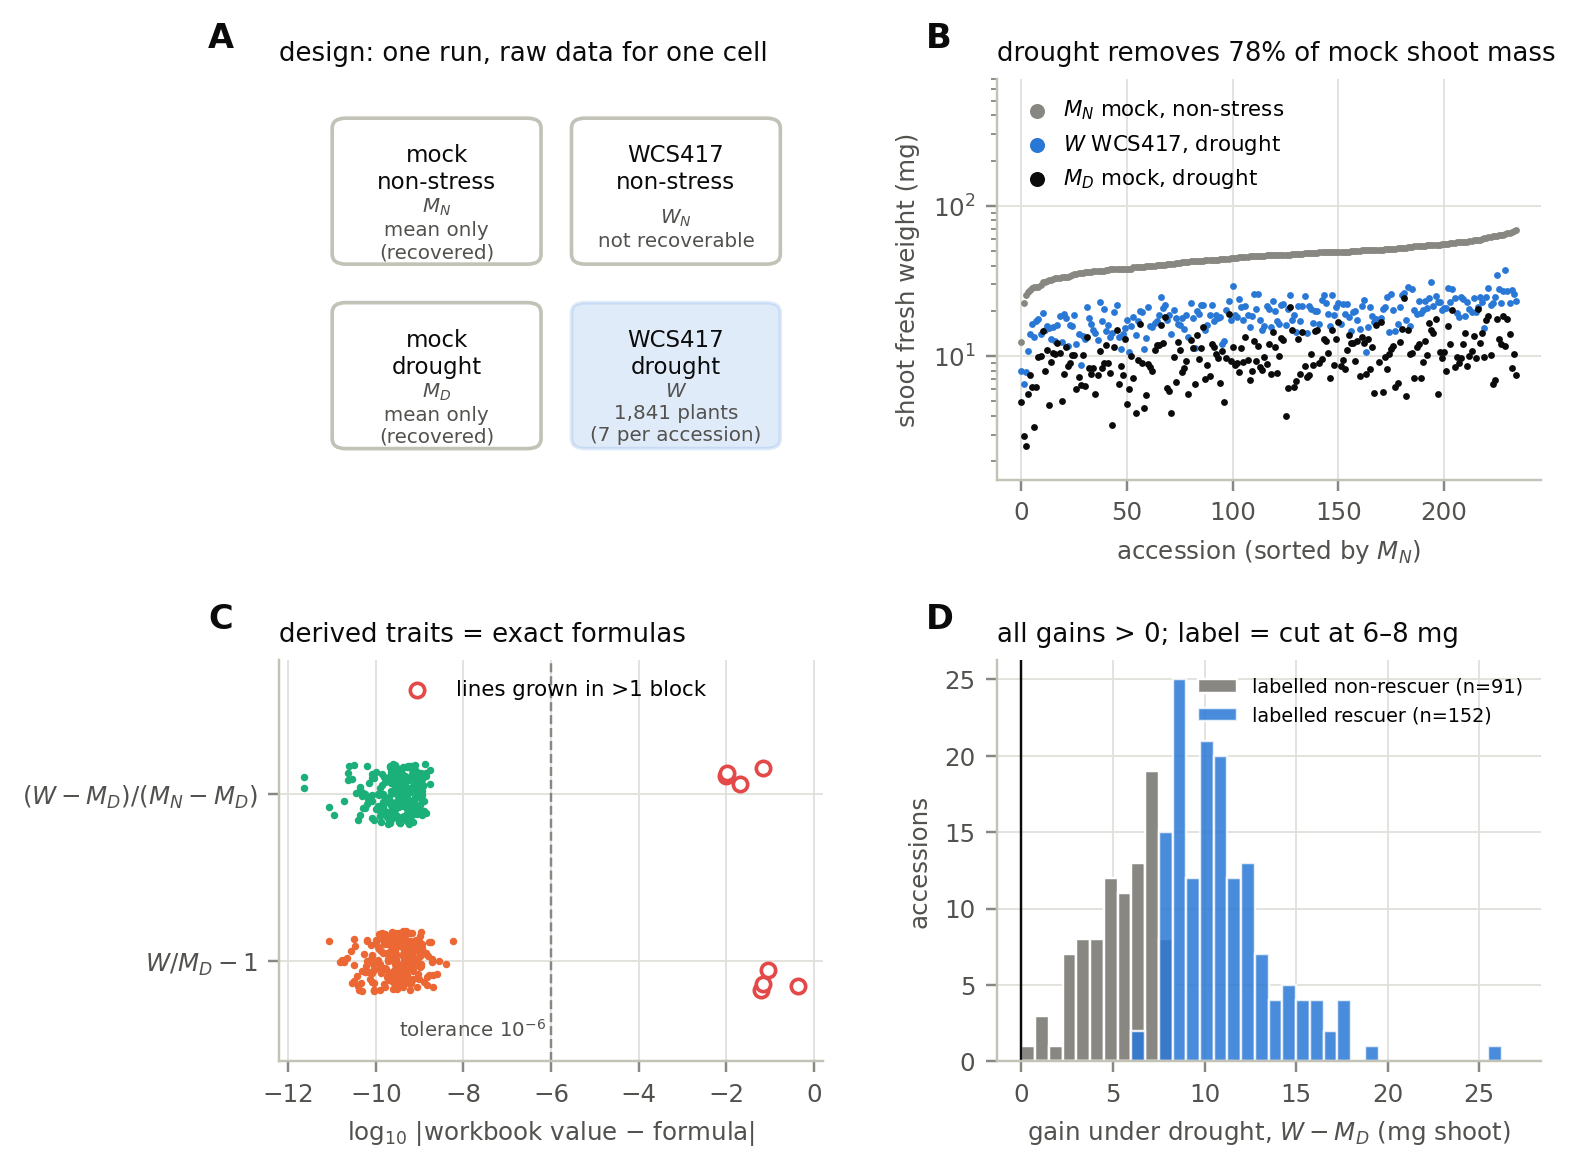
\includegraphics[width=\textwidth]{panel_1_audit.png}
    \column{0.40\textwidth}
    \small
    \begin{itemize}
      \item The formulas fit all 235 complete accessions to $10^{-10}$:
        \begin{itemize}
          \item rescue $= (W-\MD)/(\MN-\MD)$
          \item increase $= W/\MD - 1$
        \end{itemize}
      \item The second workbook \key{confirms} the reconstructed mock means by measurement.
      \item Three corrections:
        \begin{itemize}
          \item \% loss uses \bad{no inoculated plants}.
          \item Table~2 ``tolerance'' is actually loss.
          \item ``Non-rescuer'' is a cut at 6--8\,mg; every accession gains.
        \end{itemize}
    \end{itemize}
  \end{columns}
\end{frame}

% =====================================================================
\begin{frame}{The readings disagree about who rescues best}
  \begin{columns}[c]
    \column{0.58\textwidth}
    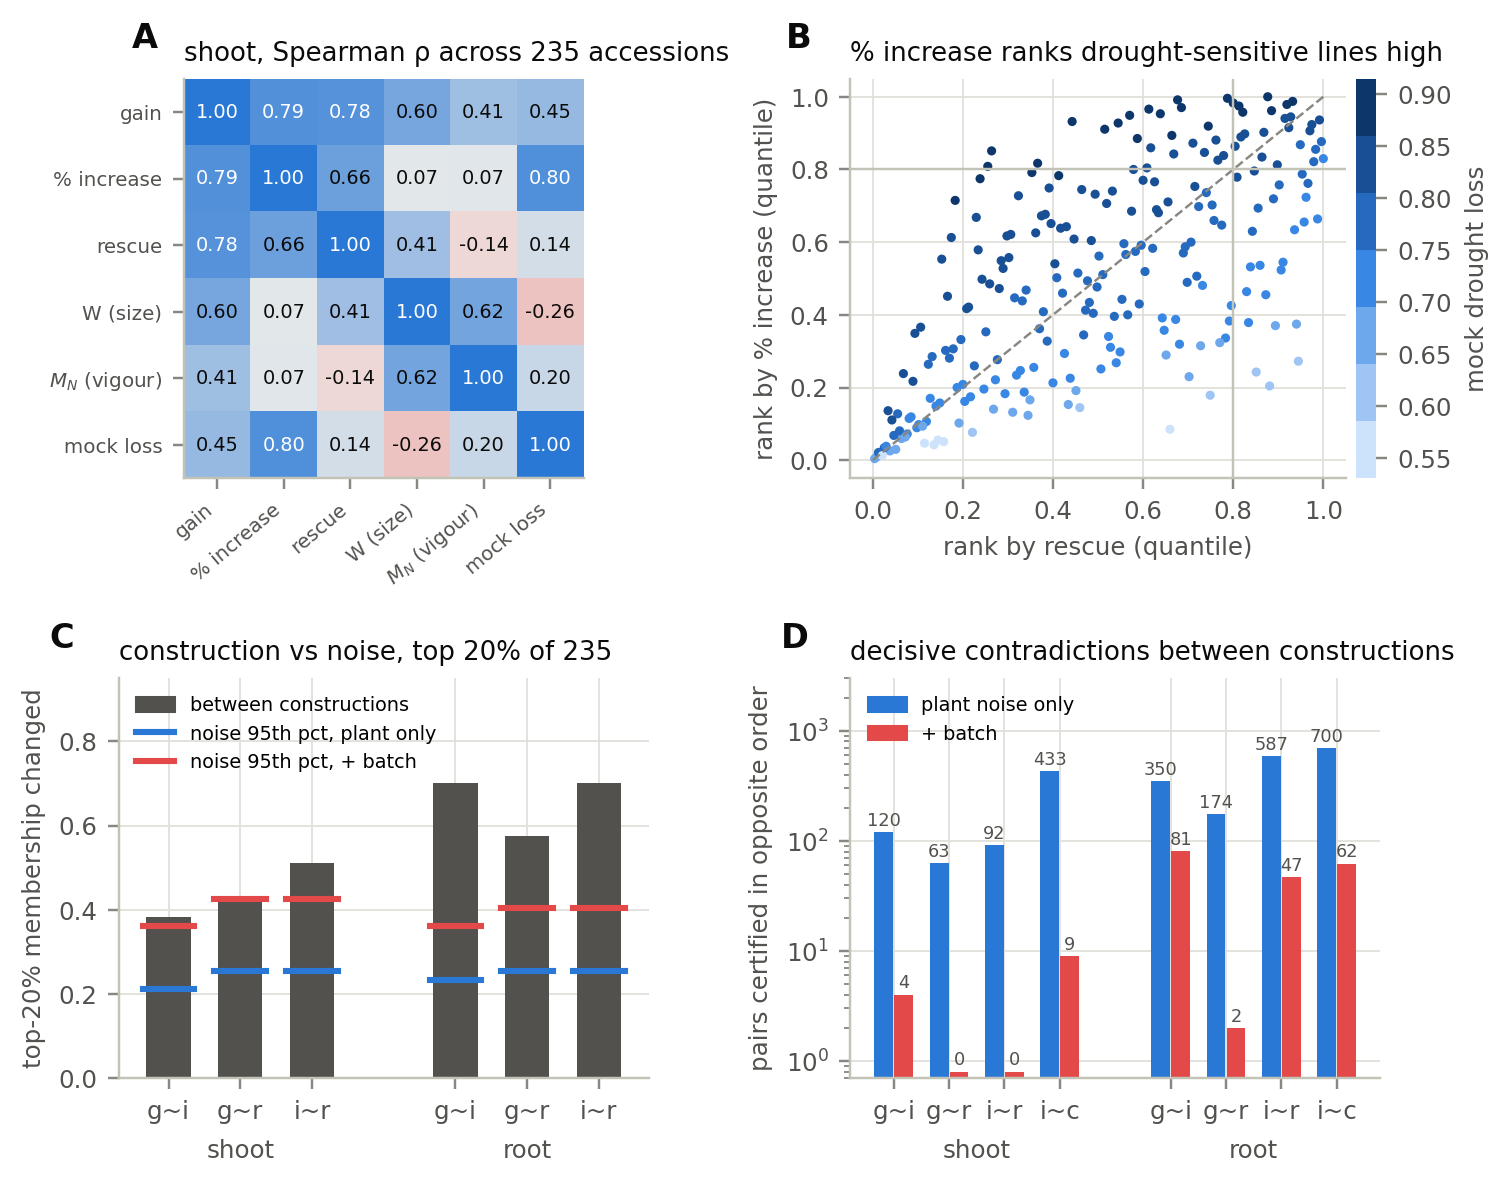
\includegraphics[width=\textwidth]{panel_3_dependence.png}
    \column{0.40\textwidth}
    \small
    \begin{itemize}
      \item Top-20\% overlap between readings:
        \begin{itemize}
          \item Jaccard 0.32--0.45 in shoot;
          \item 0.18--0.27 in root.
        \end{itemize}
      \item Each reading carries a different nuisance:
        \begin{itemize}
          \item \% increase ranks \key{drought sensitivity} ($\rho=0.80$);
          \item gain tracks plant size ($\rho=0.60$);
          \item rescue is the least loaded, but the noisiest.
        \end{itemize}
      \item Under plant noise, two readings certify up to 700 pairs of accessions
        in \bad{opposite order}.
    \end{itemize}
  \end{columns}
\end{frame}

% =====================================================================
\begin{frame}{Letting the data choose the reading}
  \begin{columns}[c]
    \column{0.58\textwidth}
    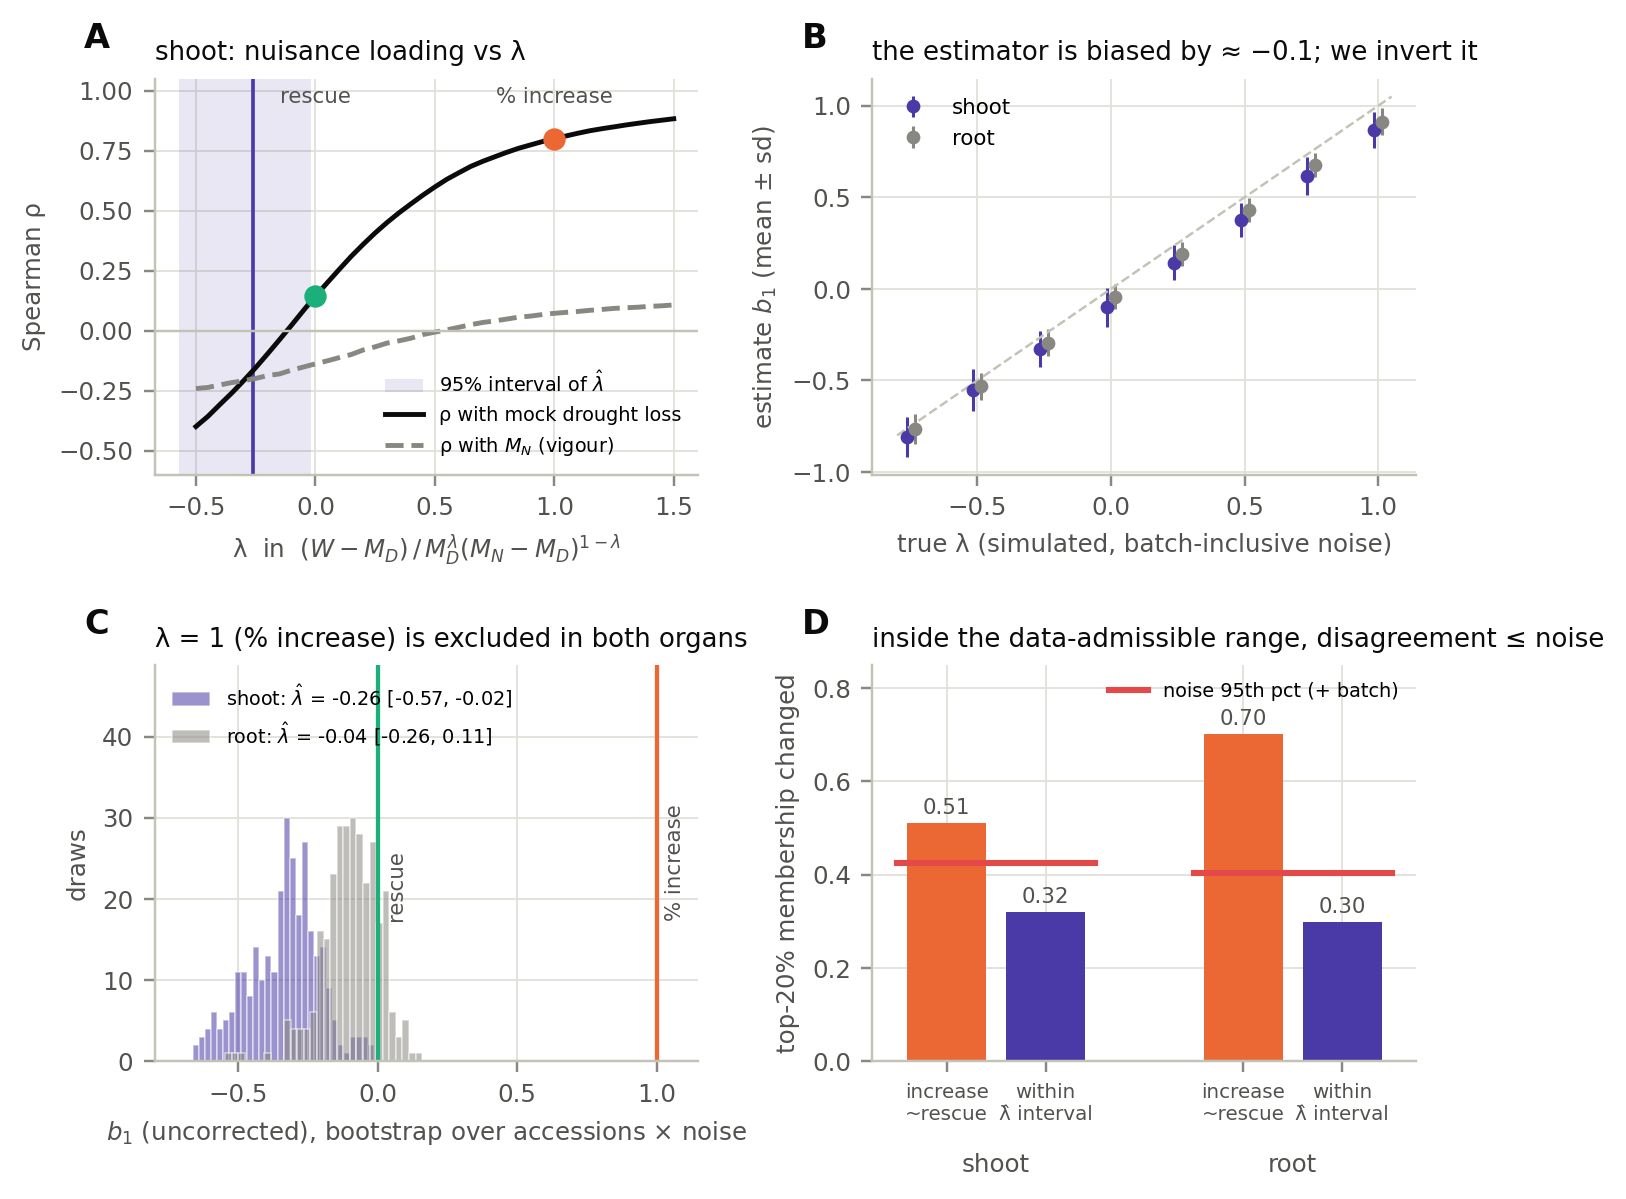
\includegraphics[width=\textwidth]{panel_4_canonical.png}
    \column{0.40\textwidth}
    \small
    \[
      f_\lambda=\frac{W-\MD}{\MD^{\lambda}(\MN-\MD)^{1-\lambda}}
    \]
    \begin{itemize}
      \item $\lambda=1$ is \% increase; $\lambda=0$ is rescue.
      \item Choosing $\lambda$ means choosing a mechanism: does WCS417 multiply the
        stressed biomass, or restore a share of what drought removed?
      \item Estimated from the data: shoot $\hat\lambda\approx-0.15$, root $\approx0.05$.
        \bad{\% increase is excluded}; rescue lies at or inside the interval.
    \end{itemize}
  \end{columns}
\end{frame}

% =====================================================================
\begin{frame}{Candidate genes, sorted by what they are loci \emph{for}}
  \begin{columns}[c]
    \column{0.58\textwidth}
    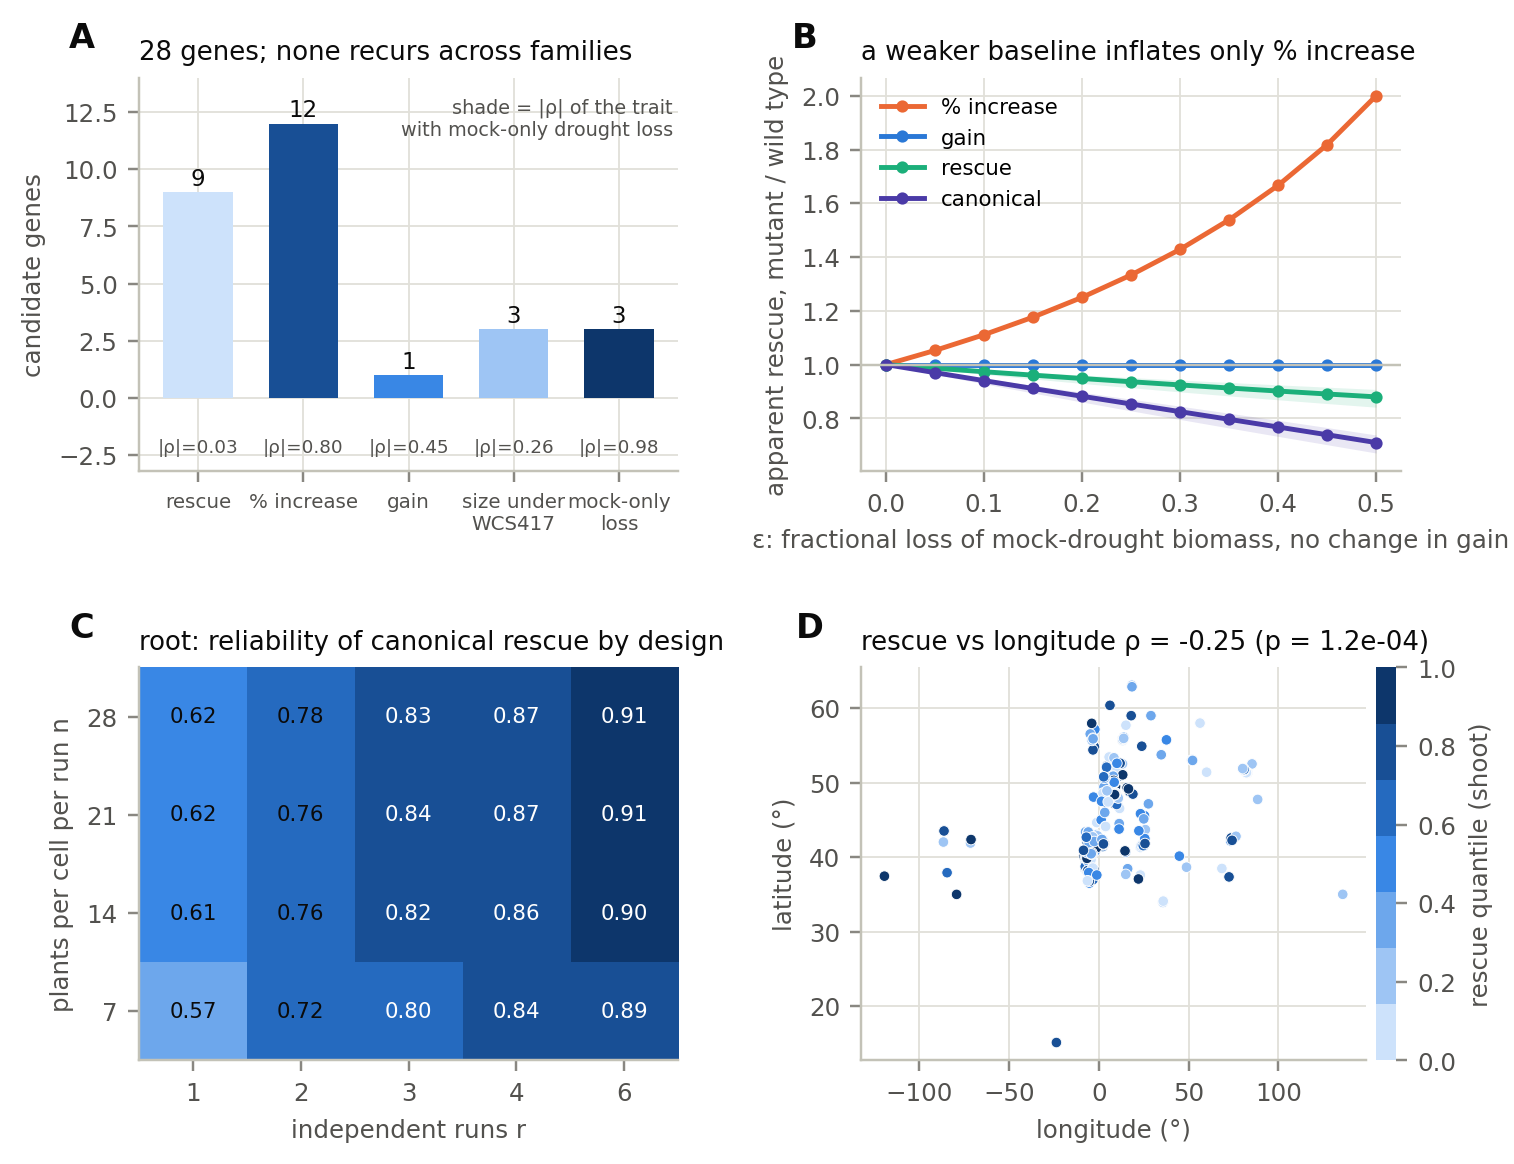
\includegraphics[width=\textwidth]{panel_6_consequences.png}
    \column{0.40\textwidth}
    \small
    \begin{itemize}
      \item 28 genes; \key{none} recurs across trait families.
      \item By the trait family each was found in:
        \begin{itemize}
          \item 3 from mock-only loss: MORN4, TPS21, AT2G07213;
          \item 12 from \% increase: at risk of being drought-sensitivity loci;
          \item 9 from rescue.
        \end{itemize}
      \item Mutant check (panel B): a mutant that is only weaker under drought looks up to
        $2\times$ ``better rescued'' under \% increase, and unchanged under gain.
    \end{itemize}
  \end{columns}
\end{frame}

% =====================================================================
\section{Part II --- does it replicate?}
\begin{frame}
  \centering\Large\color{accent}\textbf{Part II}\\[0.4em]
  \normalsize\color{black} The full per-plant workbook: three runs and a non-stress control
\end{frame}

% =====================================================================
\begin{frame}{The replicate runs at a glance}
  \centering
  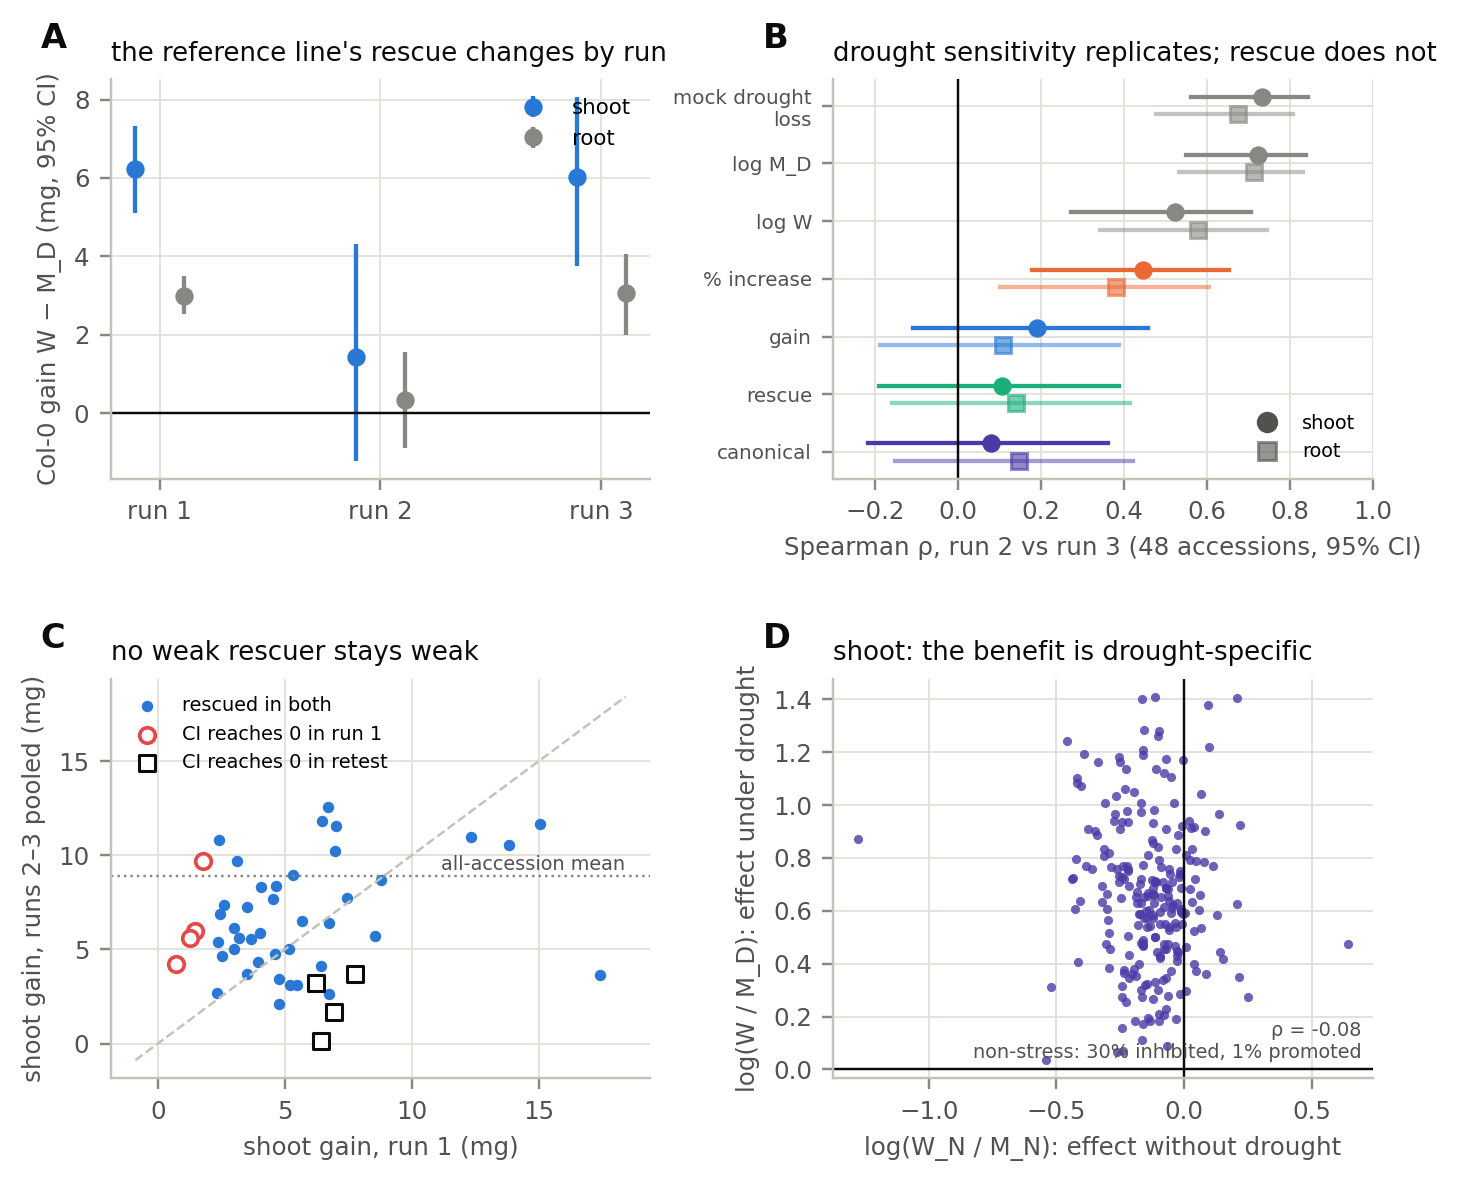
\includegraphics[height=0.84\textheight]{panel_7_full_workbook.png}
\end{frame}

% =====================================================================
\begin{frame}{The reference line is not stable across runs}
  \begin{columns}[c]
    \column{0.5\textwidth}
    \centering
    \begin{tabular}{lccc}
      \toprule
      Col-0, shoot & run 1 & run 2 & run 3 \\
      \midrule
      gain (mg) & 6.2 & \bad{1.4} & 6.0 \\
      95\% CI & [5.1, 7.3] & [$-1.2$, 4.3] & [3.8, 8.1] \\
      \bottomrule
    \end{tabular}
    \\[0.8em]
    \small Root: 3.0, \bad{0.3}, 3.1\,mg.
    \column{0.46\textwidth}
    \begin{itemize}
      \item Same genotype, same protocol.
      \item In run 2, Col-0 would have been called a \bad{non-rescuer}.
      \item Within a run, batch is largest in mock-drought plants
        (block CV 0.18).
      \item Without drought, mock and inoculated trays moved together ($r=0.66$--$0.88$),
        so batch cancelled. Under drought they did not ($r\approx0$).
    \end{itemize}
  \end{columns}
\end{frame}

% =====================================================================
\begin{frame}{What survives an independent rerun?}
  \small Spearman $\rho$ between run 2 and run 3 for the same 48 accessions. No modelling
  is involved, and neither run was used to select them.
  \vspace{0.5em}
  \begin{center}
  \begin{tabular}{lcc}
    \toprule
    & shoot $\rho$ [95\% CI] & root $\rho$ [95\% CI] \\
    \midrule
    mock drought loss (no bacterium) & \key{0.73} [0.56, 0.84] & \key{0.68} [0.48, 0.81] \\
    $\log \MD$ & 0.72 [0.55, 0.84] & 0.71 [0.53, 0.83] \\
    $\log W$ & 0.52 [0.27, 0.71] & 0.58 [0.34, 0.74] \\
    \% increase & 0.45 [0.18, 0.65] & 0.38 [0.10, 0.61] \\
    gain & \bad{0.19} [$-0.11$, 0.46] & \bad{0.11} [$-0.19$, 0.39] \\
    rescue & \bad{0.11} [$-0.19$, 0.39] & \bad{0.14} [$-0.16$, 0.42] \\
    \bottomrule
  \end{tabular}
  \end{center}
  \vspace{0.3em}
  \begin{itemize}
    \item \key{Drought sensitivity replicates; the benefit from WCS417 does not.}
    \item \% increase does moderately well only because it ranks drought sensitivity.
  \end{itemize}
\end{frame}

% =====================================================================
\begin{frame}{No weak rescuer stays weak}
  \begin{itemize}
    \item 50 apparent weak rescuers were regrown twice.
    \item Gain compatible with zero:
      \begin{itemize}
        \item 5 accessions in run 1;
        \item 4 \emph{different} accessions in the pooled retest;
        \item \key{0 in both}, and no negative retest estimate.
      \end{itemize}
    \item Per-1, the best loss-of-rescue candidate, was rescued in both retests:
      5.3 and 3.2\,mg, both intervals above zero.
    \item The regrown accessions moved 26\% (shoot) and 32\% (root) of the way back to the
      population mean. This is regression to the mean after selecting on one noisy run.
  \end{itemize}
  \vspace{0.6em}
  \begin{block}{Conclusion}
    There is no confirmed loss-of-rescue accession. This is consistent with the
    \key{redundancy} hypothesis: WCS417 helps essentially every genotype.
  \end{block}
\end{frame}

% =====================================================================
\begin{frame}{The benefit is specific to drought}
  \begin{columns}[T]
    \column{0.5\textwidth}
    \textbf{Without drought}
    \begin{itemize}
      \item WCS417 slightly \bad{inhibits} shoot growth: mean $-12\%$.
      \item 30\% of accessions are significantly inhibited; 1\% promoted.
      \item Root is unchanged on average.
    \end{itemize}
    \column{0.5\textwidth}
    \textbf{Under drought}
    \begin{itemize}
      \item 95\% (shoot) and 99\% (root) of accessions are promoted.
      \item The effect is \key{uncorrelated} with the non-stress effect
        ($\rho=-0.08$, $-0.01$).
    \end{itemize}
  \end{columns}
  \vspace{0.8em}
  \begin{itemize}
    \item This is not general growth promotion carried into drought. It differs from
      plate assays without stress (Wintermans et al.\ 2016), where nearly all accessions
      were promoted.
    \item The inoculation $\times$ water interaction is not a clean phenotype either: it
      correlates 0.79--0.82 with drought loss.
  \end{itemize}
\end{frame}

% =====================================================================
\begin{frame}{How finely can the screen rank accessions?}
  \begin{center}
  \begin{tabular}{lcc}
    \toprule
    Canonical rescue, shoot & median certifiable margin & tiers resolved \\
    \midrule
    measured plant noise & 2.0 SD & 8 \\
    + within-run batch (Col-0 blocks) & 3.3 SD & 3 \\
    + run-to-run noise (runs 2 vs 3) & \bad{4.6 SD} & \bad{2} \\
    \bottomrule
  \end{tabular}
  \end{center}
  \begin{itemize}
    \item ``Certifiable margin'': the smallest difference at which two accessions could be
      declared equivalent, in units of the between-accession spread.
    \item The screen can say that accessions differ. It cannot say that they rescue
      equally.
    \item Once realistic run-to-run noise is included, a single run separates
      \key{2--3 levels} of rescue, not 235 ranks. Root resolves 3.
  \end{itemize}
\end{frame}

% =====================================================================
\begin{frame}{What this means for the GWAS}
  \begin{enumerate}
    \item \key{The current candidate genes are hits on a single-run phenotype.}
      \begin{itemize}
        \item Rescue has a run-to-run reliability of about 0.1--0.2.
        \item Expect poor replication, except for drought-sensitivity loci.
      \end{itemize}
    \item \key{Drought sensitivity is the solid result.}
      \begin{itemize}
        \item Mock drought loss replicates at $\rho\approx0.7$.
        \item A drought-sensitivity GWAS is publishable now; the phenotype table is
          prepared.
      \end{itemize}
    \item \key{A rescue GWAS needs a phenotype averaged over several runs.}
      \begin{itemize}
        \item Spearman--Brown: reliability 0.6 needs about 6 runs (at 0.2) to 14 runs
          (at 0.1).
      \end{itemize}
    \item \key{The biology survives and sharpens.}
      \begin{itemize}
        \item The benefit is drought-specific and reliably positive.
        \item Accessions do not reproducibly differ in how much they are helped.
      \end{itemize}
  \end{enumerate}
\end{frame}

% =====================================================================
\begin{frame}{Design for the next screen}
  \begin{itemize}
    \item \key{Independent runs, not more plants.}
      \begin{itemize}
        \item A second run is worth more than four times the plants in one run.
      \end{itemize}
    \item \key{Co-locate mock and inoculated plants} of each accession on the same tray.
      \begin{itemize}
        \item This already happened without drought, and the batch cancelled.
      \end{itemize}
    \item \key{Control drought severity between runs.}
      \begin{itemize}
        \item Col-0 mock-drought biomass varied 16--22\,mg between runs.
      \end{itemize}
    \item \key{Keep Col-0 in every block}, record block membership, and model block.
    \item \key{Fix the phenotype before mapping}: loss-normalised rescue, averaged over
      runs, with kinship and (in root) $\log\MN$ as covariates.
    \item \key{Grow mutants in the same run as their wild type}, and report gain and rescue
      alongside \% increase.
  \end{itemize}
\end{frame}

% =====================================================================
\begin{frame}{Open questions for the lab}
  \begin{enumerate}
    \item Were runs 2 and 3 chosen to confirm the apparent non-rescuers?
    \item Under drought, were mock and inoculated plants on separate trays?
    \item How was drought severity set and monitored in each run?
    \item Was the non-stress experiment a single run, and grown at the same time as
      run 1?
    \item Were the iron-uptake mutants grown alongside their wild type, and which metric
      showed ``higher rescue''?
    \item Can we get the genotypes (1001 Genomes IDs are already in the sheet), so the
      drought-sensitivity GWAS can be rerun with kinship?
  \end{enumerate}
\end{frame}

% =====================================================================
\begin{frame}{Caveats}
  \small
  \begin{itemize}
    \item The replicated accessions were selected as weak rescuers. Their run-1 gains still
      spread 91\% as widely as the full panel's.
    \item Two runs on 48 accessions give wide intervals; the tables show them.
    \item Non-stress was grown once, so its run-to-run reproducibility is unknown.
    \item No genotypes were available: no association was rerun or tested.
    \item The $\lambda$ family is a model. In root, the data reject its exact scale
      invariance.
    \item Bootstrap-based quantities move slightly between reruns. Accessions near a
      threshold (e.g.\ Choto-1, Wl-0) can flip.
  \end{itemize}
  \vspace{0.8em}
  \footnotesize Code: \texttt{validation/experiments.py} (E1--E12) and
  \texttt{experiments\_full.py} (F1--F7), seed 417; every number is read from
  \texttt{results/*.json}.
\end{frame}

\end{document}
